\documentclass[12pt,letter]{article}
\usepackage{amsmath}
\usepackage{amssymb}	% packages that allow mathematical formatting
\usepackage{graphicx}
%\graphicspath{{../Code/02_Graphs/}}
\usepackage{setspace}	% package that allows you to change spacing
\usepackage{fullpage}	% package that specifies normal margins
\usepackage{microtype}
\usepackage{amsthm}
\newcommand{\argmin}{\operatornamewithlimits{argmin}}
\renewcommand\qedsymbol{$\blacksquare$}
\usepackage{listings,lstautogobble}
\lstset{language=R,
	autogobble=true,
	breaklines=true
}
\usepackage{pgfplotstable} %include csv tables
\usepackage{float} %allows specific table positionings
\usepackage{color}
\renewcommand\qedsymbol{$\blacksquare$}

\usepackage[left=2.5cm, right=2.5cm, top=2cm, bottom = 3cm]{geometry}
	

\begin{document}
\title{FNCE 924 --- Problem Set 2}
\author{Felix Nockher and Patrick Shultz}
\date{\today}
\maketitle 
\section*{Part I: Asset Prices with Complete Markets}
Consider the Lucas (1978) asset pricing model and assume consumers have CRRA preferences $\bigg(u(c_t) = \frac{c_t^{1-\gamma}}{1-\gamma}\bigg)$ with risk aversion $\gamma$ and discount rate $\beta$. Suppose that income/dividend/endowment growth obeys 
\begin{equation*}
	\log(y_{t+1}/y_t) = g + \epsilon_{t+1}
\end{equation*}
where $\epsilon_{t+1}$ is i.i.d. $N(0, \sigma^2)$
\paragraph{a)}Compute the market price of a risk free bond that is purchased in period $t$ and pays exactly one unit of consumption in period $t+1$. \\

The Lucas asset pricing model implies identical agents that can trade a stock and a bond. Shares in the aggregate endowment are given by $\theta^s(S^t) \in \Theta^s$ and shares of the bond are given by $\theta^b(S^t)\in\Theta^b$. Each household solves the following problem
\begin{equation*}
	V(\theta^s, \theta^b, S) = \max_{\{c, \theta^{'s}, \theta^{'b}\}}\left\{u(c) + \beta \int_{S}V(\theta^{'s}, \theta^{'b}, S')F(S, dS')\right\}
\end{equation*}
subject to the constraint $c + \theta^{'s} Q^s + \theta^{'b}Q^b = \left[y + Q^s\right]\theta^s + \theta^b$. Letting $\lambda(S)$ denote the Lagrange multiplier in state $S$, we get the following first order conditions
\begin{equation*}
\begin{split}
	u_c(c(\theta^s, \theta^b, S))-\lambda(S) &= 0\\
	\beta \int_{S}V_{\theta^b}(\theta^{'s}, \theta^{'b}, S')F(S, dS') - \lambda(S)Q^b(S) &=0\\
\end{split}
\end{equation*}
The bond price is given by combining the Envelope condition $\bigg(V_{\theta^b} = \lambda(S) = u_c(c)\bigg)$ and the FOC
\begin{equation*}
\begin{split}
	Q^b(S) &= \beta E_t\left[\frac{u_c(c')}{u_c(c)}\right]\\
	&= \beta E_t\left[\left(\frac{c'}{c}\right)^{-\gamma}\right]\\
	&= \beta E_t\left[\exp\left\{-\gamma \log\left(\frac{c'}{c}\right) \right\}\right]\\
	& = \beta \exp\left\{-\gamma g + \frac{1}{2}\gamma^2\sigma^2\right\}
\end{split}
\end{equation*}
where the final equality holds because in equilibrium $c_t =y_t$ and by the properties of log-normally distributed variables. 
\paragraph{b)} Next, compute the market price, $Q_j^b$, of a risk free bond that is purchased in period $t$ and pays exactly one unit of consumption in period $t+j$ for any maturity $j$. \\

The pricing kernel from time $t$ to time $j$ is given by 
\begin{equation*}
	M_{t, t+j} = \beta^j\frac{u_c(c_{t+j})}{u_c(c_t)}
\end{equation*}
so the price of the bond is given by 
\begin{equation*}
\begin{split}
	Q^b_{t+j} &= E_t\left[M_{t+j}\right]\\
	&= \beta^j E_t\left[\left(\frac{c_{t+j}}{c_t}\right)^{-\gamma}\right]\\
	&= \beta^j E_t\left[\left(\frac{c_{t+j}}{c_t}\right)^{-\gamma}\left(\frac{c_{t+j}}{c_{t+j-1}}\right)^{-\gamma}...\left(\frac{c_{t+1}}{c_{t}}\right)^{-\gamma}\right]\\
	&= \beta^j\left(\exp\left(j(-\gamma g + \frac{1}{2}\gamma^2 \sigma^2)\right)\right)
\end{split}
\end{equation*}
where the final equality holds again by $c_t = y_t$ in equilibrium and properties of log-normal variables. 
\paragraph{c)}
We can make the income/ dividend/ endowment growth process have a time-varying mean.
\begin{equation*}
log(y_{t+1}/y_t) \sim N(g_{t,t+1},\sigma^2)
\end{equation*}
where $g_{t,t+1}$ stands for the growth from $t$ to $t+1$ and could follow an AR(1) process:
\begin{equation}\label{ARprocess}
g_{t,t+1} = (1-\varphi)\bar{g}+\varphi g_t + \sigma_g^2 \epsilon_{t+1}
\end{equation}
with $\epsilon \stackrel{iid}{\sim} N(0,1)$ and $\varphi \in (-1,1)$.

Then the time $t$ price of a bond paying 1 unit of consumption for sure at time $t+j$ would be:
\begin{align*}
Q^B_j 	&= \beta^j E_t\left[\frac{u_c(c_{t+j})}{u_c(c_t)}\right]\\
		&= \beta^j E_t\left[\left(\frac{c_{t+j}}{c_t}\right)^{-\gamma}\right]\\
		&= \beta^j E_t\left[exp\left\lbrace - \gamma log\left(\frac{c_{t+j}}{c_t}\right)\right\rbrace\right] \\
		&= \beta^j exp\left\lbrace E_t\left[- \gamma log\left(\frac{c_{t+j}}{c_t}\right)\right] + \frac{1}{2}Var_t\left[- \gamma log\left(\frac{c_{t+j}}{c_t}\right)\right]\right\rbrace &\text{due to log normality}\\
		&= \beta^j exp\left\lbrace E_t\left[- \gamma log\left(\frac{y_{t+j}}{y_t}\right)\right] + \frac{1}{2}Var_t\left[- \gamma log\left(\frac{y_{t+j}}{y_t}\right)\right]\right\rbrace &\text{due to Lucas (1978) resource constraint}\\
\end{align*}
Since we defined the process of log endowment growth above as the AR(1) process in equation \ref{ARprocess} we can then recursively solve for the two terms:
\begin{align*}
E_t\left[log\left(\frac{y_{t+j}}{y_t}\right)\right] 	&= E_t\left[g_{t,t+j}\right]\\
														&= \sum_{i=0}^{j-1}\varphi^i (1-\varphi)\bar{g} + \varphi^i g_t\\
Var_t\left[log\left(\frac{y_{t+j}}{y_t}\right)\right]	&= Var_t\left[g_{t,t+j}\right]\\
														&= Var_t\left[\sum_{i=0}^{j-1}\varphi^i \sigma_g \epsilon_{t+1+i}\right] &\text{already omitting constant terms}\\
														&= \sigma^2_g \sum_{i=0}^{j-1}\varphi^{2i} &\text{due to iid'ness of $\epsilon$}
\end{align*}
Then the time $t$ price of a bond paying 1 unit of consumption for sure at time $t+1$ is
\begin{equation}
Q^B_j = \beta^j exp\left\lbrace - \gamma \left[ \sum_{i=0}^{j-1}\varphi^i (1-\varphi)\bar{g} + \varphi^i g_t \right]+ \frac{1}{2}\left[\gamma^2 \sigma^2_g \sum_{i=0}^{j-1}\varphi^{2i}\right]\right\rbrace
\end{equation}
Consequently, the yield of maturity j is:
\begin{equation}
R^b_j = (Q^B_j)^{-1/j} = \beta^{-1} exp\left\lbrace - \gamma \left[ \sum_{i=0}^{j-1}\varphi^i (1-\varphi)\bar{g} + \varphi^i g_t \right]+ \frac{1}{2}\left[\gamma^2 \sigma^2_g \sum_{i=0}^{j-1}\varphi^{2i}\right]\right\rbrace^{-1/j}
\end{equation}
We see that due to the stationarity of the mean process $g_t$ the further we look into the future ($j \to \infty$), the less the most current observation $g_t$ impacts our outlook and the closer we get to the long-term mean. Thereby the rate of convergence (i.e. the slope of the yield curve) depends on the persistence of the process which is in turn determined by how close $\varphi$ is to $|1|$.
For instance with the following parameters $\gamma = 2,\ \bar{g}= 0.1,\ \sigma_g = 0.3,\ g_t = 0.03$ we get the following yield curves:

\begin{figure}[H]
	\centering
	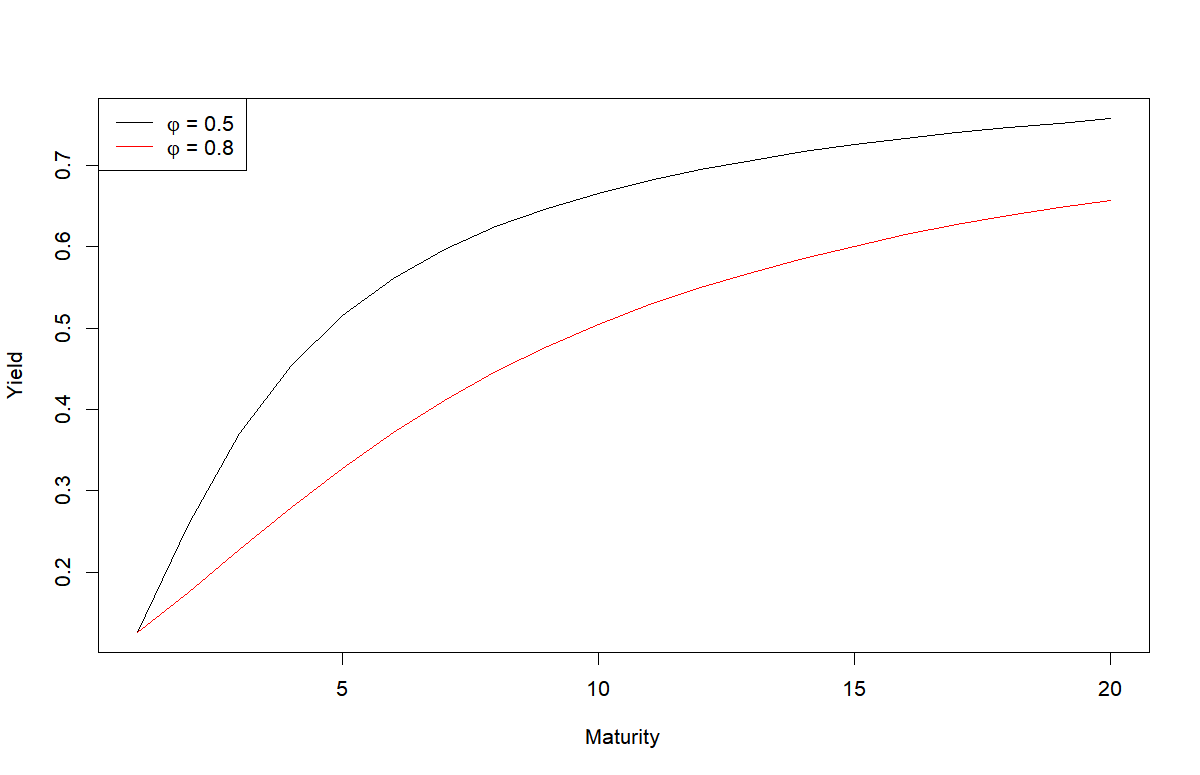
\includegraphics[trim={0 0 0 1.5cm},clip,width=\textwidth]{I_1d_YieldCurve}
	\caption{Implied yield curve with time-varying mean of the endowment growth process}
	\label{Figure I.1d}
\end{figure}
\section*{Part II: Computing Asset Prices in Incomplete Markets}
Economy is populated with 5500 households with identical CRRA preferences with risk aversion equal to 2 and discount factor $\beta = 0.97$. Suppose financial markets are incomplete in the sense that each household can only invest in a one period risk free bond, that pays gross interest rate $R$. The budget constraint for each household $i$ is given by 
\begin{equation*}
	k_{t+1} + c_t = y_t + Rk_{t+1}
\end{equation*}
where the borrowing constraint is defined as $k_{t+1}\geq-1$. Assume household income follows $\log y_t = \rho \log y_{t-1} + \sigma(1-\rho^2)^{1/2}\epsilon_t$ with $\rho =0.6$, $\sigma = 0.35$, and $\epsilon$ is normal iid with mean 0 and variance 1. 
\paragraph{a)} Suppose $R=1.01$. Solve the problem of each household numerically. Plot the optimal policies for consumption and capital accumulation against the current level of capital for two different levels of current income, $y$. \\

First, we note that the AR(1) process of log income has a mean of zero and variance of $\frac{\sqrt{1-\rho ^2} \sigma }{1-\rho ^2} = 0.4375$. Using these moments, we can use the Tauchen-Hussey method to determine optimal grid points for income. \\

Given the set up above, we calculate the value functions in Figure \ref{fig:value_functions} and policy functions in Figure \ref{fig:policy_functions}.
\begin{figure}[H]
	\centering
	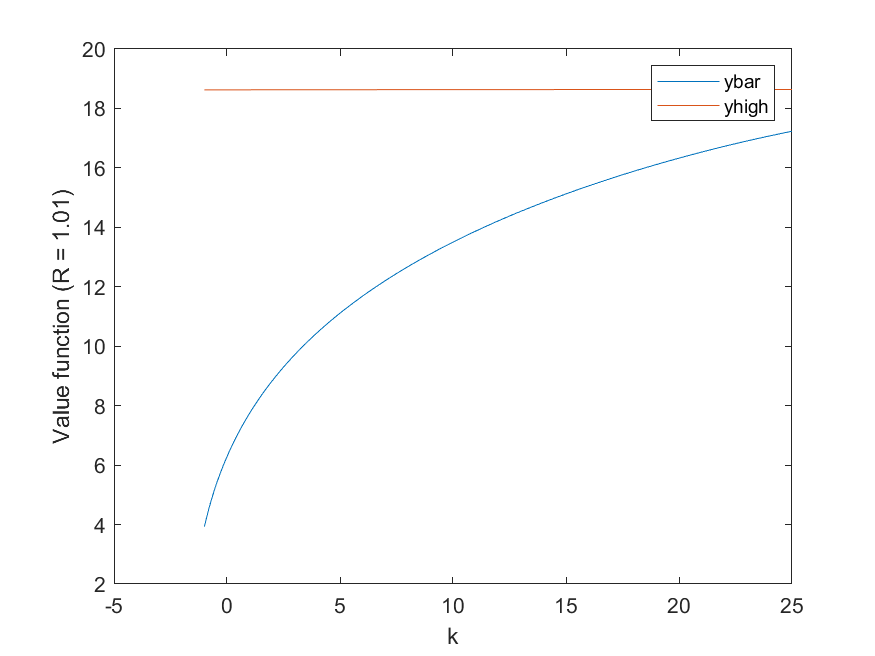
\includegraphics[scale=0.75]{value_functions_gridpoints501.png}
	\caption{Value functions with $R = 1.01$}
	\label{fig:value_functions}
\end{figure}
\begin{figure}[H]
	\centering
	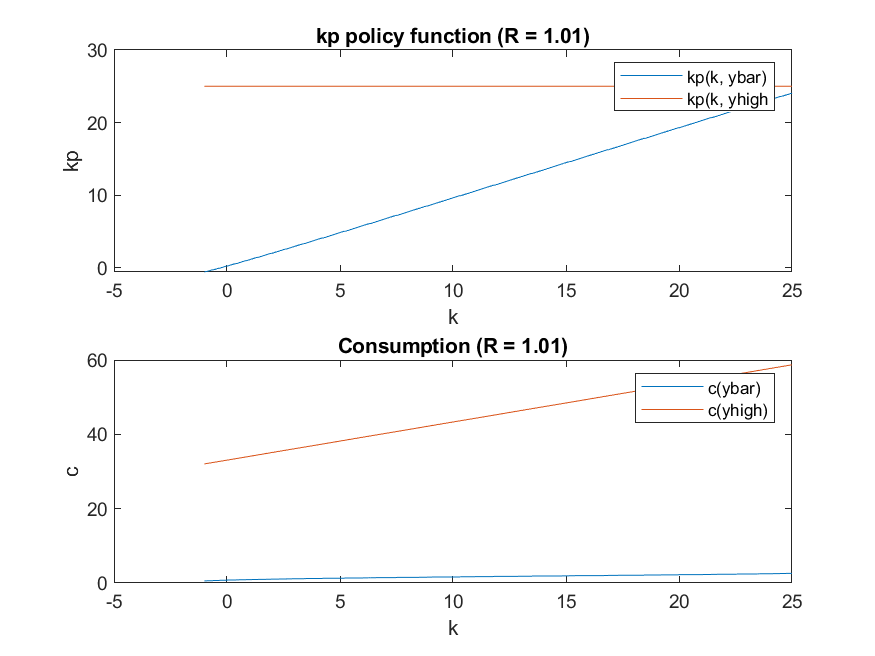
\includegraphics[scale=0.75]{c_and_k_gridpoints501.png}
	\caption{Policy functions with $R=1.01$}
	\label{fig:policy_functions}
\end{figure}
\paragraph{b)} Simulate the economy for 2500 periods. After dropping the first 500 observations compute the aggregate demand for assets in th economy in each period by summing over the optimal choices $k'(k, y)$. \\

We now simulate the economy for 5500 consumers to see what the aggregate demand for assets looks like over time with $R = 1.01$. We see that there is excess demand for borrowing. Thus, the interest rate is too low and we need to increase it to give our agents an incentive to save. 


\begin{figure}[H]
	\centering
	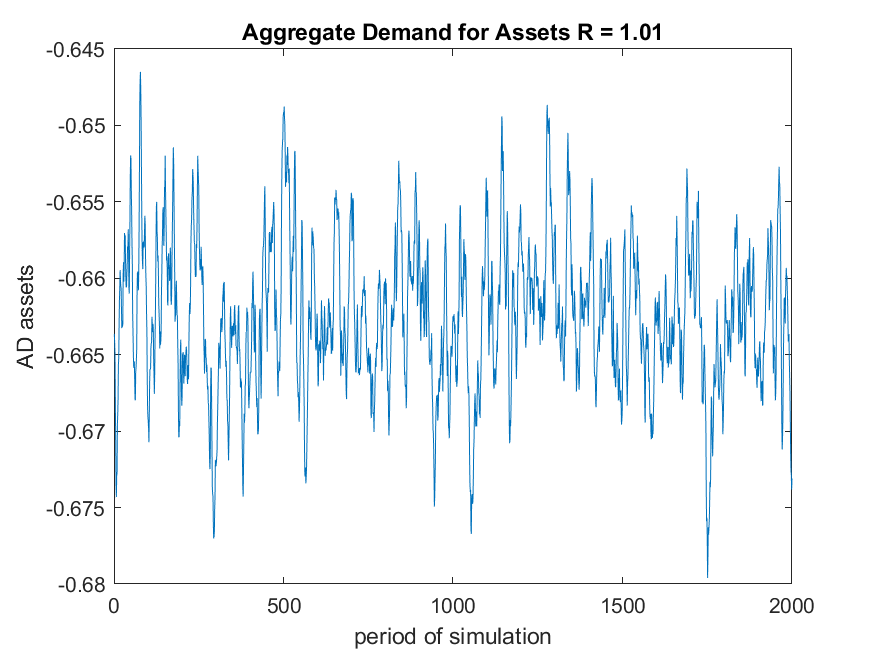
\includegraphics[scale=0.75]{aggregate_demand.png}
	\caption{Aggregate demand with $R=1.01$}
	\label{fig:agg_demand_high_r}
\end{figure}

In Figure \ref{fig:agg_demand_equilibrium}, we see that an interest rate of $R = 1.02525$ generates a time series where the mean aggregate demand across households fluctuates around 0 for the entire sample. The sample average is also near zero, so we consider this our equilibrium rate. 
\begin{figure}[H]
	\centering
	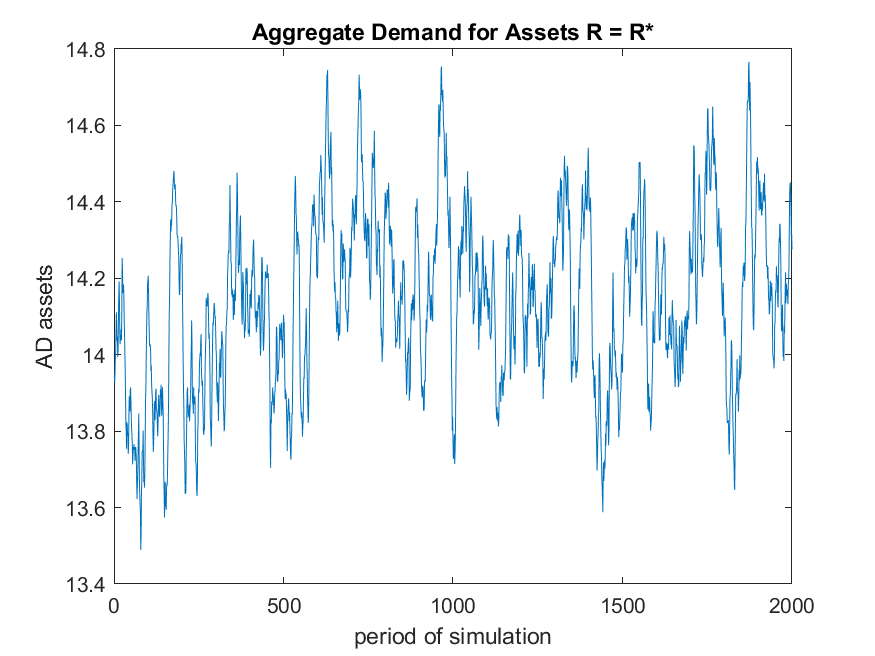
\includegraphics[scale=0.75]{aggregate_demand_equilibrium.png}
	\caption{Aggregate demand with $R=R^*$, where $R^*$ denotes the equilibrium rate}
	\label{fig:agg_demand_equilibrium}
\end{figure}

In Figure \ref{fig:agg_demand_bconst}, we see that decreasing the borrowing constraint allows households to borrow more on average, which causes the the average aggregate demand for savings to be negative. Thus, the interest rate is too low given these parameters. 
\begin{figure}[H]
	\centering
	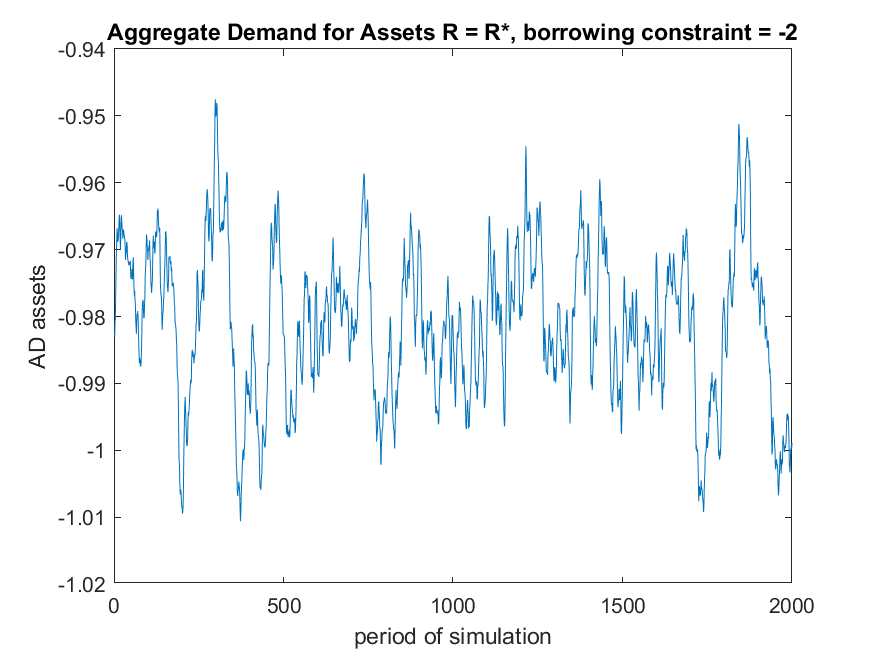
\includegraphics[scale=0.75]{aggregate_demand_bconst.png}
	\caption{Aggregate demand with $R=R^*$, but $b = -2$.}
	\label{fig:agg_demand_bconst}
\end{figure}
\section*{Part III: Investment and Asset Prices}
The profit function, adjustment cost, and capital accumulation equations for an infinitely lived firm are given by the linear homogeneous expressions
\begin{equation*}
	\begin{split}
	\pi_t &= a_tk_t\\
	\phi_t &= \gamma\left[\frac{i_t}{k_t}-\eta_t\right]^2k_t\\
	i_t &= k_{t+1} - (1-\delta)k_t
	\end{split}
\end{equation*}

\paragraph{a)} Compute the one period gross return to the accumulation of physical capital $R^K_{t, t+1}$. \\

The firm's problem is given by 
\begin{equation*}
	v_0 = \max_{\{d_t, k_{t+1}, i_t\}_{t=0}^\infty} E_0\left[\sum_{t=0}^{\infty}M_{0, t}d_t\right]
\end{equation*}
subject to the constraints $d_t = \pi_t - i_t - \phi_t$ and $i_t = k_{t+1} - (1- \delta)k_t$.  Thus, the firm's problem is to maximize the following expression
\begin{equation*}
		v_0 = \max_{\{k_{t+1}, i_t\}_{t=0}^\infty}E_0\left[\sum_{t=0}^{\infty}M_{0, t}\bigg(\pi_t(a_t, k_t) -i_t(k_t, k_{t+1}) - \phi(i_t, k_t)\bigg)\right]
\end{equation*}
subject to the constraint $i_t = k_{t+1} - (1- \delta)k_t$. Noting that the that the total derivatives of the adjustment cost function at times $t$ and $t+1$ with respect to $k_{t+1}$ take the forms of $\frac{\partial \phi_t}{\partial i_t}\frac{\partial i_t}{\partial k_{t+1}}$ and $ \frac{\partial \phi_{t+1}}{\partial k_{t+1}} + \frac{\partial \phi_{t+1}}{\partial i_{t+1}}\frac{\partial i_{t+1}}{\partial k_{t+1}}$, respectively, we get the following first order condition with respect to $k_{t+1}$

\begin{equation*}
	E_0\left[M_{0, t} \left(\frac{\partial i_t}{\partial k_{t+1}} + \frac{\partial \phi_t}{\partial i_t}\frac{\partial i_t}{\partial k_{t+1}}\right)\right] = E_0\left[M_{0, t+1}\bigg(\frac{\partial \pi_{t+1}}{\partial k_{t+1}} -\frac{\partial i_{t+1}}{\partial k_{t+1}} - \frac{\partial \phi_{t+1}}{\partial k_{t+1}} - \frac{\partial \phi_{t+1}}{\partial i_{t+1}}\frac{\partial i_{t+1}}{\partial k_{t+1}}\bigg)\right]
\end{equation*}
The first order condition equates marginal cost of increasing capital stock today with the expected marginal benefit to this increase in capital. Taking expectations at time $t$, we get the Euler equation 

\begin{equation*}
	1 = E_t \left[M_{t, t+1}\left(\frac{\frac{\partial \pi_{t+1}}{\partial k_{t+1}} -\frac{\partial i_{t+1}}{\partial k_{t+1}} - \frac{\partial \phi_{t+1}}{\partial k_{t+1}} - \frac{\partial \phi_{t+1}}{\partial i_{t+1}}\frac{\partial i_{t+1}}{\partial k_{t+1}}}{\frac{\partial i_t}{\partial k_{t+1}} + \frac{\partial \phi_t}{\partial i_t}\frac{\partial i_t}{\partial k_{t+1}}}\right)\right]
\end{equation*}

Computing the partial derivatives gives
\begin{equation*}
\begin{split}
1 &= E_t \left[M_{t, t+1}\left(\frac{a_{t+1} + (1-\delta) - \bigg(\gamma  \left(\frac{i_{t+1}}{k_{t+1}}-\eta_{t+1} \right)^2-\frac{2 \gamma  i_{t+1}}{k_{t+1}} \left(\frac{i_{t+1}}{k_{t+1}}-\eta_{t+1} \right)\bigg) - \bigg(2 \gamma  \left(\frac{i_{t+1}}{k_{t+1}}-\eta_{t+1} \right) (\delta-1)\bigg)}{1 + 2 \gamma  \left(\frac{i_t}{k_t}-\eta_t \right)}\right)\right]\\
&=E_t \left[M_{t, t+1}\left(\frac{a_{t+1}-\gamma  (-\delta +\eta_{t+1}+1)^2-\delta +\frac{\gamma k_{t+2}^2}{k_{t+1}^2}+1}{1 + 2 \gamma  \left(\frac{i_t}{k_t}-\eta_t \right)}\right)\right]\\
\end{split}
\end{equation*}
where the second equality holds by substituting out $i_{t+1}$ and simplification. Thus, we have 
\begin{equation*}
	R^k_{t+1} = \frac{a_{t+1}-\gamma  (\eta_{t+1}+1-\delta)^2 +\frac{\gamma k_{t+2}^2}{k_{t+1}^2}+1-\delta}{1 + 2 \gamma  \left(\frac{i_t}{k_t}-\eta_t \right)}
\end{equation*}
\paragraph{b)} Recall the expression for firm value is derived from the fact that $E_t\left[M_{t, t+1}R^s_{t, t+1}\right] = 1$, where $R^S_{t, t+1}$ is the return to the firm's equity. Show that under the assumptions of linear homogeneity, we can establish that $R^S_{t, t+1} = R^K_{t, t+1}$.\\

Define return to the firm's equity as 
\begin{equation*}
	R^S_{t, t+1} = \frac{v^e_{t+1}+d_{t+1}}{v_t^e}
\end{equation*}
and conjecture that the ex-dividend value of the firm has the form $v^e_t = q_t k_{t+1}$. Thus, return to the firm's equity has the form 
\begin{equation}
	R^s_{t, t+1} =\frac{q_{t+1}k_{t+2}+ d_{t+1}}{q_t k_{t+1}}
	\label{eq:return_to_equity}
\end{equation} 
With smooth adjustment costs, we solve the problem in two stages. First, we determine the optimal amount of investment conditional on the shadow value of capital. Second, we determine the shadow value of capital. We define $q_t$ as the multiplier on the capital accumulation in period $t$, so our problem becomes 
\begin{equation*}
	\mathcal{L} = \sum_{s=0}^{\infty}M_{0, t+s}\bigg[\pi(a_{t+s}, k_{t+s}) - i_{t+s}-\phi(i_{t+s}, k_{t+s}) + q_{t+s}\bigg(i_{t+s}-k_{t+s+1}-(1-\delta)k_{t+s}\bigg)\bigg]
\end{equation*}
We  consider the optimal investment decision conditional on knowing the shadow value of capital. Optimal investment solves the static problem
\begin{equation*}
\psi(a_t, k_t) = \max_{i_t}\left[(q_t-1)i_t - \phi(i_t, k_t)\right]
\end{equation*}
Solving this problem, we get that the optimal investment rate is
\begin{equation}
\frac{q_{t}-1}{2\gamma} + \eta_t = \frac{i_t}{k_t} \implies q_t = 1 + 2\gamma\left(\frac{i_t}{k_t}-\eta_t\right)
\label{eq:opt_inv}
\end{equation}
Plugging Equation \ref{eq:opt_inv} into Equation \ref{eq:return_to_equity}, we get 
\begin{equation*}
\begin{split}
		R^s_{t, t+1} &=\frac{\left(1 + 2\gamma\left(\frac{i_{t+1}}{k_{t+1}}-\eta_{t+1}\right)\right)k_{t+2}+ d_{t+1}}{1 + 2\gamma\left(\frac{i_t}{k_t}-\eta_{t+1}\right)k_{t+1}}\\
		&= \frac{\left(1 + 2\gamma\left(\frac{i_{t+1}}{k_{t+1}}-\eta_t\right)\right)k_{t+2}+ \pi_{t+1} - i_{t+1}- \phi(i_{t+1}, k_{t+1})}{(1 + 2\gamma\left(\frac{i_t}{k_t}-\eta_t\right))k_{t+1}}\\
		& = \frac{k_{t+1} \left(a_{t+1}-\gamma  (\eta_{t+1}+1-\delta)^2-\delta +1\right)+\frac{\gamma k_{t+2}^2}{k_{t+1}}}{(1 + 2\gamma\left(\frac{i_t}{k_t}-\eta_t\right))k_{t+1}}\\
		& = R^k_{t, t+1}
\end{split}
\end{equation*}
\end{document}